\documentclass[12pt]{article}
\usepackage[a4paper, margin=0.75in]{geometry}
\usepackage[document]{ragged2e}
\usepackage{graphicx}
\usepackage{multicol}
\graphicspath{ {./images/} }
\usepackage{enumerate}
\usepackage{framed}
\usepackage{amsmath,amsfonts,amsthm,thmtools,amssymb,mathtools,commath}
\usepackage{physics}
\usepackage{tikz}
\usetikzlibrary{mindmap}
\usepackage{caption}
\usepackage{xcolor}
\usepackage[most]{tcolorbox}
\usepackage{cleveref}


%%%%%%%%%%%%%%%%
%  Definition  %
%%%%%%%%%%%%%%%%
\tcbuselibrary{theorems,skins,hooks}
\newtcbtheorem[number within=subsection]{definition}{Definition}%
{
    % theorem style=definition,
    enhanced,
	before skip=2mm,after skip=2mm, colback=cyan!5,colframe=cyan!80!black,boxrule=0.5mm,
	attach boxed title to top left={xshift=1cm,yshift*=1mm-\tcboxedtitleheight},
	boxed title style={frame code={
					\path[fill=cyan]
					([yshift=-1mm,xshift=-1mm]frame.north west)
					arc[start angle=0,end angle=180,radius=1mm]
					([yshift=-1mm,xshift=1mm]frame.north east)
					arc[start angle=180,end angle=0,radius=1mm];
					\path[left color=cyan!30!black,right color=cyan!30!black,
						middle color=cyan!50!black]
					([xshift=-2mm]frame.north west) -- ([xshift=2mm]frame.north east)
					[rounded corners=1mm]-- ([xshift=1mm,yshift=-1mm]frame.north east)
					-- (frame.south east) -- (frame.south west)
					-- ([xshift=-1mm,yshift=-1mm]frame.north west)
					[sharp corners]-- cycle;
				},interior engine=empty,
		},
	fonttitle=\bfseries,
	title={#2},#1
}{def}


%%%%%%%%%%%%%
%  Theorem  %
%%%%%%%%%%%%%
\tcbuselibrary{theorems,skins,hooks}
\newtcbtheorem[use counter from=definition]{theorem}{Theorem}%
{
    theorem style=plain,
    enhanced,
    colframe=green,
    boxrule=1pt,
    titlerule=0mm,
    toptitle=1mm,
    bottomtitle=1mm,
    fonttitle=\bfseries,
    fontupper=\mdseries\itshape,
    coltitle=green!30!black,
    colbacktitle=cyan!15!white,
    colback=green!10,
    description font=\bfseries\sffamily
}{thrm}


%%%%%%%%%%%%%%
% Corollary  %
%%%%%%%%%%%%%%
 \tcbuselibrary{theorems,skins}
 \newtcbtheorem[use counter from=theorem]{corollary}{Corollary}%
 {
    theorem style=plain,
    enhanced,
    colframe=green,
    frame hidden,
    titlerule=0mm,
    toptitle=1mm,
    bottomtitle=1mm,
    fonttitle=\bfseries,
    fontupper=\mdseries\itshape,
    coltitle=green!30!black,
    colbacktitle=cyan!15!white,
    colback=green!10,
    description font=\bfseries\sffamily
 }{corl}


%%%%%%%%%%%%%
%  Example  %
%%%%%%%%%%%%%
\tcbuselibrary{theorems,skins,hooks}
\newtcbtheorem[number within=section]{example}{Example}%
{
	enhanced,
	breakable,
	colback = gray!5,
	frame hidden,
	boxrule = 0sp,
	borderline west = {2pt}{0pt}{gray},
	sharp corners,
	detach title,
	before upper = \tcbtitle\par\smallskip,
    coltitle=gray!70!black,
	fonttitle = \bfseries\sffamily,
	description font = \mdseries\bfseries
}
{xmp}


%%%%%%%%%%%%%%
%  Exercise  %
%%%%%%%%%%%%%%
\tcbuselibrary{theorems,skins,hooks}
\newtcbtheorem[number within=section]{exercise}{Exercise}%
{
    enhanced,
    breakable,
    colback=black!5,
    colframe=black!30,
    left=0.5em,
    before skip=10pt,
    after skip=10pt,
    boxrule=0pt,
    boxsep=0pt,
    arc=0pt,
    outer arc=0pt,
    borderline west={3pt}{0pt}{black!30},
}{exc}

%%%%%%%%%%
%  Note  %
%%%%%%%%%%
\usetikzlibrary{arrows,calc,shadows.blur}
\tcbuselibrary{skins}
\newtcolorbox{note}[1][]{%
	enhanced jigsaw,
	colback=gray!20!white,%
	colframe=gray!80!black,
	size=small,
	boxrule=1pt,
	title=\textbf{Note:-},
	halign title=flush center,
	coltitle=black,
	breakable,
	drop shadow=black!50!white,
	attach boxed title to top left={xshift=1cm,yshift=-\tcboxedtitleheight/2,yshifttext=-\tcboxedtitleheight/2},
	minipage boxed title=1.5cm,
	boxed title style={%
			colback=white,
			size=fbox,
			boxrule=1pt,
			boxsep=2pt,
			underlay={%
					\coordinate (dotA) at ($(interior.west) + (-0.5pt,0)$);
					\coordinate (dotB) at ($(interior.east) + (0.5pt,0)$);
					\begin{scope}
						\clip (interior.north west) rectangle ([xshift=3ex]interior.east);
						\filldraw [white, blur shadow={shadow opacity=60, shadow yshift=-.75ex}, rounded corners=2pt] (interior.north west) rectangle (interior.south east);
					\end{scope}
					\begin{scope}[gray!80!black]
						\fill (dotA) circle (2pt);
						\fill (dotB) circle (2pt);
					\end{scope}
				},
		},
	#1,
}


\title{
    \textbf{Experiment 11} \\
    \textbf{Experiment on Band Reject Filter} \\
}

\author{
    Turja Roy \\
    ID: 2108052
}
\date{}

\begin{document}
\maketitle

\section{Objective}
\begin{enumerate}
    \item To determine the Band reject filter frequency response of an RC circuit. 
    \item To measure the cut off frequency and observe the attenuation rate. 
    \item To compare the graph of simulation data and practical data.
\end{enumerate}

\section{Apparatus}
\begin{multicols}{2}
    \begin{enumerate}
        \item Resistors
        \item Capacitors
        \item Oscilloscope
        \item Breadboard
    \end{enumerate}
    \columnbreak
    \begin{enumerate}
        \item Wires
        \item Function Generator
        \item DC Power Supply
        \item Multimeter
    \end{enumerate}
\end{multicols}

\section{Circuit Diagram}
\begin{figure}[h]
    \centering
    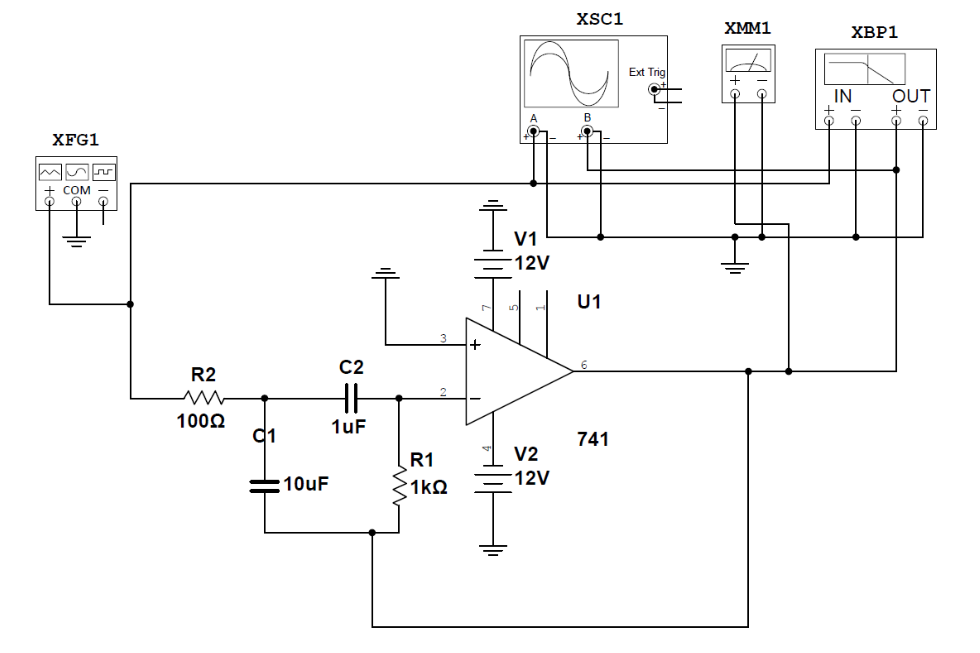
\includegraphics[width=0.7\textwidth]{BPF.png}
    \caption{Band Reject Filter RC Circuit}
\end{figure}

\section{Result Analysis}
The bandstop filter is formed when a low pass filter and a high pass filter are connected in parallel with each other. The main function of the bandstop filter is eliminating or stopping the particular band of frequencies. The bandstop filter is also referred with some other names like band-reject or notch or band elimination filter. As discussed previously, For high pass filter there will be one cut off frequency, low pass filter also has one cut off frequency but this bandpass and bandstop filters have two cut off frequencies. \\~\\

This band stop filter will reject a particular range of frequencies which are there in between the two cut off frequencies. It allows the frequencies which are above the high cut off frequency and the below the low cut off frequencies. These two cut off frequencies are determined based on the value of components used in the design of the circuit. This filter has a stopband and two passbands. \\~\\

When the signal is given an input, a low pass filter allows the low frequencies to pass through the circuit and a high pass filter allows the high frequencies to pass through the circuit. \\~\\

This is the block diagram of the bandstop filter. Low pass filter and high pass filter are connected in parallel. There is some difference between ideal and practical conditions while working with the filter. This difference is due to the switching mechanism of a capacitor. The frequency response can be clearly explained in the above figure. \\~\\

The set of frequency for which the filter acts as a short circuit is depending on the lower and higher cut off frequencies. These cut off frequencies are dependent on the components and its value used while designing. According to the design, the transfer function determines the component values.

\newpage
\subsection{Data Table}

\begin{table}[h!]
    \centering
    \caption{Practical Data of Band Reject Filter}
    \begin{tabular}{rrrrr}
        \hline
        F &    log F &  Vin &  Vout &         Av \\
        \hline
        1.0 & 0.000000 &    2 & 0.033 & -35.650321 \\
        1.5 & 0.176091 &    2 & 0.033 & -35.650321 \\
        2.0 & 0.301030 &    2 & 0.330 & -15.650321 \\
        2.5 & 0.397940 &    2 & 0.031 & -36.193366 \\
        3.0 & 0.477121 &    2 & 0.031 & -36.193366 \\
        3.5 & 0.544068 &    2 & 0.031 & -36.193366 \\
        4.0 & 0.602060 &    2 & 0.032 & -35.917600 \\
        4.5 & 0.653213 &    2 & 0.032 & -35.917600 \\
        5.0 & 0.698970 &    2 & 0.032 & -35.917600 \\
        5.5 & 0.740363 &    2 & 0.035 & -35.139239 \\
        6.0 & 0.778151 &    2 & 0.400 & -13.979400 \\
        6.5 & 0.812913 &    2 & 0.710 &  -8.995433 \\
        7.0 & 0.845098 &    2 & 0.159 & -21.992657 \\
        7.5 & 0.875061 &    2 & 0.238 & -18.489061 \\
        8.0 & 0.903090 &    2 & 0.278 & -17.139704 \\
        8.5 & 0.929419 &    2 & 0.312 & -16.137508 \\
        9.0 & 0.954243 &    2 & 0.372 & -14.609741 \\
        10.0 & 1.000000 &    2 & 0.650 &  -9.762333 \\
        20.0 & 1.301030 &    2 & 0.794 &  -8.024190 \\
        30.0 & 1.477121 &    2 & 0.886 &  -7.071925 \\
        40.0 & 1.602060 &    2 & 0.951 &  -6.456990 \\
        50.0 & 1.698970 &    2 & 0.988 &  -6.125461 \\
        60.0 & 1.778151 &    2 & 1.031 &  -5.755427 \\
        100.0 & 2.000000 &    2 & 1.239 &  -4.159174 \\
        500.0 & 2.698970 &    2 & 1.241 &  -4.145164 \\
        1000.0 & 3.000000 &    2 & 1.222 &  -4.279176 \\
        5000.0 & 3.698970 &    2 & 1.189 &  -4.516963 \\
        10000.0 & 4.000000 &    2 & 1.140 &  -4.882503 \\
        20000.0 & 4.301030 &    2 & 1.104 &  -5.161218 \\
        30000.0 & 4.477121 &    2 & 1.063 &  -5.489935 \\
        40000.0 & 4.602060 &    2 & 1.017 &  -5.874181 \\
        50000.0 & 4.698970 &    2 & 0.740 &  -8.635966 \\
        100000.0 & 5.000000 &    2 & 0.448 & -12.995040 \\
        200000.0 & 5.301030 &    2 & 0.176 & -21.110347 \\
        300000.0 & 5.477121 &    2 & 0.070 & -29.118639 \\
        400000.0 & 5.602060 &    2 & 0.040 & -33.979400 \\
        500000.0 & 5.698970 &    2 & 0.035 & -35.139239 \\
        1000000.0 & 6.000000 &    2 & 0.056 & -31.056839 \\
        2000000.0 & 6.301030 &    2 & 0.450 & -12.956350 \\
        3000000.0 & 6.477121 &    2 & 0.450 & -12.956350 \\
        5000000.0 & 6.698970 &    2 & 0.450 & -12.956350 \\
        \hline
    \end{tabular}
\end{table}

\newpage
\subsection{Graph}

\begin{figure}[h]
    \centering
    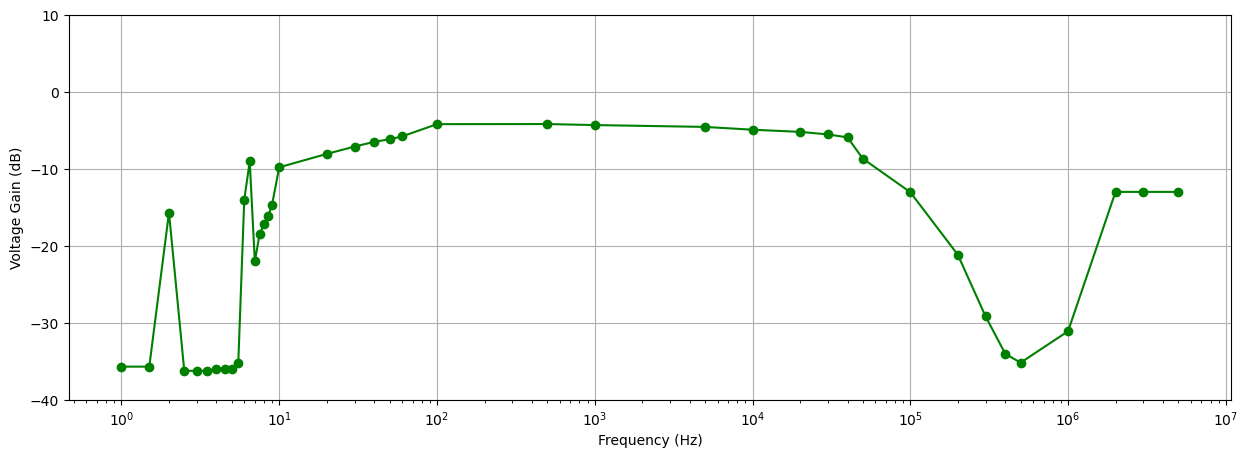
\includegraphics[width=0.8\textwidth]{BPF_Graph.png}
    \caption{Frequency Response of Band Reject Filter}
\end{figure}

In this graph we were seen that at the low frequency the the gain was highest .After increasing the frequency randomly we were seen that this graph block the highier frequency and pass the lower frequency and then after more increasing the frequency we were seen that after suuden time the graph was decrease by increasing the frequency and then after sudden time the filter look like the high pass filter.And that was condition of Band reject filter.

\section{Discussion}
The bandstop filter is formed when a low pass filter and a high pass filter are connected in parallel with each other. The main function of the bandstop filter is eliminating or stopping the particular band of frequencies. The bandstop filter is also referred with some other names like band-reject or notch or band elimination filter. As discussed previously, For high pass filter there will be one cut off frequency, low pass filter also has one cut off frequency but this bandpass and bandstop filters have two cut off frequencies. \\~\\

\end{document}

